
\documentclass[aspectratio=169]{beamer}
\usepackage[square,numbers]{natbib}
\usepackage{/home/hx/latex/mytheme/UISBearmer/beamerthemeUIS}
%% macro
\input{\string~/latex/mytheme/macro/macro}
%% end macro

\bibliographystyle{apalike}
%%Tilte and [Short titile], optionally
\title[]{Computing Real Numbers with Large-Population Protocols Having a Continuum of Equilibria}
\date[]{\large{\today}}
%% The current style file does not suppor multiple authors
%% You need to have a copy of the style file to modify that.
%% See mytheme/UISBearmer/beamerthemeUIS, search author

%\author[Us]{\Large{Xiang Huang} \and \Large{Rachel Huls}}

\author[Xiang\,Huang \& Rachel.\,Huls]
{%

  \texorpdfstring{
    \begin{columns}%[onlytextwidth]
      \column{.45\linewidth}
      \centering
      Xiang Huang\\
      \href{mailto:xhuan5@uis.edu}{(xhuan5@uis.edu)}\\
      \href{https://xianghuang.org}{xianghuang.org}
      \column{.45\linewidth}
      \centering
      Rachel Huls\\
      \href{mailto:rhuls2@uis.edu}{(rhuls2@uis.edu)}
    \end{columns}
  }
  {Xiang Huang \& Rachel Huls}
}
%\institute{\inst{1} University of Us1 \and \inst{2} University of Us2}

%\author[\\\vspace{5em}\LARGE{University of Illinois Springfield}]{\Large{Xiang Huang (xhuan5@uis.edu)} \hspace{2em}Rachel Huls \hspace{10em}}
\institute{\Large{University of Illinois Springfield}} % Type in A


%% This is just to remove the annoying warning message dure to href package.
%% see:  https://tex.stackexchange.com/questions/192686/hyperref-warning-caused-by-beamer-appendix/567706#567706
%% and also: https://github.com/josephwright/beamer/issues/449
\pdfstringdefDisableCommands{%
\def\translate#1{#1}%
}
%%% end handling href warning.

\begin{document}

\begin{frame}
\maketitle
\end{frame}

\begin{frame}{Outline}
\tableofcontents
\end{frame}

\section{Background}

\begin{frame}{Why computing real numbers?}
\begin{itemize}
    \item Theoretical benchmark. (Turing 1936, computable numbers. We now consider analog models.) \pause
    \item Complicated systems not based on concrete biochemical problems. \pause
    \item Guide algorithm design.
\end{itemize}
\end{frame}

\begin{frame}[Clean]{Real numbers by Population Protocols?}

What do we mean by saying a real number is computable by a PP?

\begin{example}[Bournez et. al., 2011\footnote{Guillaume Aupy, Olivier Bournez. On the number of binary-minded individuals required to compute $\frac{1}{\sqrt{2}}$}.]
\begin{figure}[tb]
    \centering
    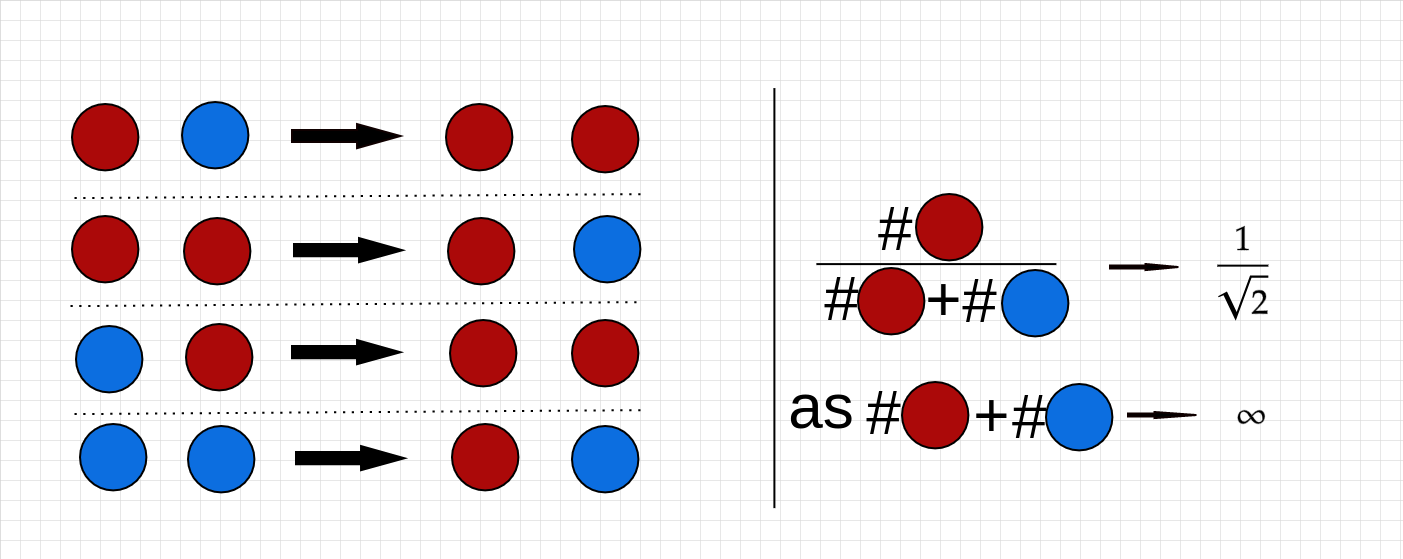
\includegraphics[scale=0.2]{ppexample1}
\end{figure}
\end{example}
\end{frame}

\begin{frame}{Basic Properties of Computable numbers}
Some basic properties:
\begin{enumerate}
    \item They are the \emph{expected} proportion of some species and hence are between 0 and 1.
    \item Total population goes to infinity. We call such population protocols ``large-population protocols'' or LPPs.
    \item Although all proportions are rationals, but the limits might not be so.
\end{enumerate} \pause
Extra requirement and property:
\begin{itemize}
    \item They systems must have finitely many equilibria.
    \item The computing result usully does not depend on initial values.
\end{itemize}

\end{frame}

\begin{frame}[Clean]{The power of LPPs with finite equilibria}
    \textbf{Question}: Can we compute $\frac{\pi}{4}$?
\pause
\begin{theorem}[Bournez et. al., 2016. (with a gap)\footnote{Olivier Bournez, Pierre Fraigniaud, and Xavier Koegler. Computing with
large populations using interactions.} ]
A number $\alpha$ is computable by a large-population protocol if and only if $\alpha$ is \emph{algebraic}.
\end{theorem}
\pause
So only numbers like  $\frac{1}{\sqrt{7}}$ and $\sqrt{3}-\sqrt{2}$; no $\frac{\pi}{4}$ and $e^{-1}$.
\end{frame}

\begin{frame}{but on the other hand ...}%here fragile is necessary in order to use the \verbatim environment
The General Purpose Analog Computer (GPAC) and Chemical Reaction Networks (CRNs) are not so boring.

\begin{theorem}[Huang, Klinge and Lathrop 2019]
    Transcendental numbers such as $\pi$, $e$, and Euler's $\gamma$ can be computed by GPAC/CRN \emph{in real time}.
\end{theorem}
\begin{itemize}
    \item Roughly, $\alpha$ is computable if there is a species $x$ such that $\lim_{t\to \infty} x(t)=\alpha$.
    \item ``In real time'' simply means we can do it quick. We are not talking about real-time computation today.
\end{itemize}
\end{frame}

\begin{frame}{An analog Church-Turing thesis}%here fragile is necessary in order to use the \verbatim environment
Church-Turing thesis: All powerful enough models are equivalent (in some sense).
\begin{quest}
    Are large-population protocols as powerful as GPACs/CRNs (in terms of computing real numbers)?
\end{quest}
Or can LPPs ``compute'' at least some transcendental numbers in some way?
\end{frame}

\begin{frame}
    \begin{figure}[tb]
        \centering
        
\includegraphics[scale=1.8]{bridge}
    \end{figure}
\end{frame}

\begin{frame}{Example of a System with a continuum of equilibria}
\begin{example}[Titus Klinge]
   Let $F(t)= \frac{1}{2}e^{e^{-t} -1}$, $E(t)= \frac{1}{2}e^{-t}$, and $G(t)$ be a function such that its derivative ``cancels'' with $E$ and $F$'s derivative.
\begin{equation*}
\text{ODE:}\hspace{0.5cm}
       \begin{cases}
        F'= -2FE\\
        E'= -E \\
        G'= 2FE + E
   \end{cases}
\text{CRN/PP:} \hspace{0.5 cm}
\begin{cases}
    \reaction{F + E}{2}{G+E}\\
    E \to G.
   \end{cases}
\end{equation*}
with initial values $F(0)=\frac{1}{2}$, $E(0)=\frac{1}{2}$, and $G(0)=0$. Clearly, $F(t)\to \frac{1}{2e}$
\end{example}
\textbf{The system has all the F-G plan as equilibria.} We know the solution so we know where the system goes.
\end{frame}


\begin{frame}[Clean]{Simulation}
    Simulation (by ppsim\footnote{David Doty and Eric Severson. Ppsim: A software package for efficiently
simulating and visualizing population protocols.})
\begin{figure}[tb]
    \centering
    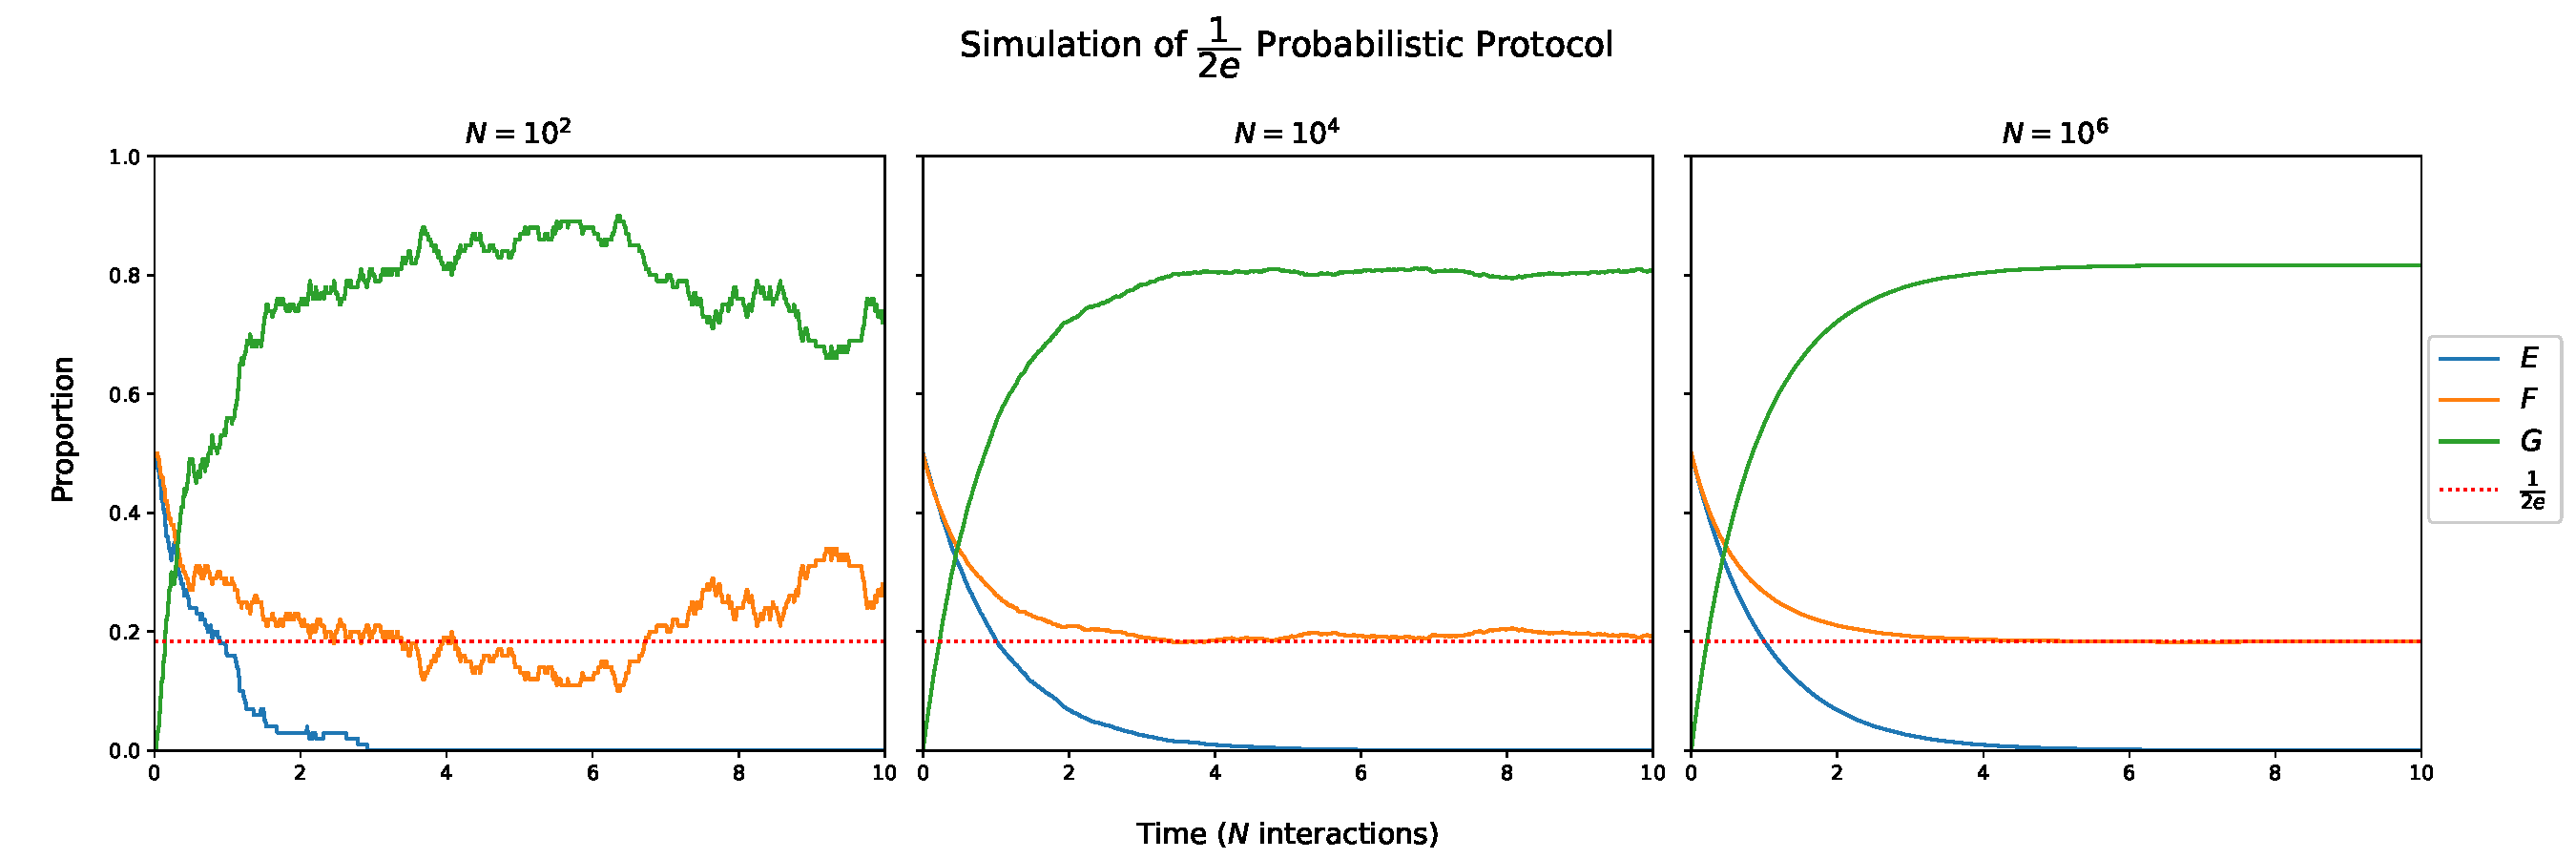
\includegraphics[scale=0.3]{half_e}
\end{figure}
\end{frame}


\begin{frame}[Clean]{Today}
\begin{todaythm}[Huang and Huls]
    LPPs compute the same set of numbers in [0,1] as GPACs
and CRNs.
\end{todaythm}
\pause
\begin{itemize}
    \item We achieve this by lifting the finitary requirement on equilibria. Now we allow systems with a continuum of equilibria.
    \item The computation results now critically depend  on initial values.
\end{itemize}\pause
Byproducts:
\begin{enumerate}
    \item We fix Bournez et. al.'s algebraic number proof.
    \item We give an algorithm turning CRNs into PPs.
    \item We can compute fancy real numbers such as Euler's $\gamma$ with population protocol!
\end{enumerate}
\end{frame}

\section{The Proof of the main theorem}
\begin{frame}[Clean]{A bridge between stochastic and continuous model}
    \begin{kurtz}[Kurtz,1972\footnote{Thomas G. Kurtz. The relationship between stochastic and deterministic models for chemical reactions.}.]
        Stochastic CRNs agree with their continuous model almost surely when population goes to infinity.
    \end{kurtz}

To simplify our discussion in this talk, we treat population protocols as two-input-two-output CRNs with deterministic mass-action semantic, under large population assumption.
\end{frame}
\begin{frame}{LPP-Computable number: Formal Definition}
\begin{definition}
    A real number $\nu$ is said to be computable by an LPP if there exists an LPP such that $\bx(t)=(x_1(t),x_2(t),\cdots,x_n(t))\in [0,1]^n$ and
    \[
        \lim_{t\to \infty}\sum_{i\in M}x_i(t)=\nu,
    \]where $M\subseteq\{1,\cdots, n\}$ represents the subset of states marked in $\bx$. Moreover, all the states $x_i$ must be initialized to some positive rational $r_i\in \mathbb{Q}\cap[0,1]$, in the sense that $\lim_{N\to \infty} x_i^{(N)}(0)=r_i$, when $x_i^{(N)}(0)$ is the initial fraction of state $i$ at the stage when the population is $N$.
\end{definition}
\end{frame}

\begin{frame}[Clean]{Polynomial Characterization of GPAC and CRN}
    \begin{columns}
        \column{0.46\textwidth}
         \vspace*{-0.6em}
        \begin{block}{GPAC/ODE}
            \vspace*{-1em}
            \begin{align*}
                &x_i^{\ \prime  }= p_i(x_1,\cdots,x_n), \\
                 &\quad\text{for $i=1,2,\cdots,n$},\\
                 &\quad\text{where $p_i$'s are polynomials.}
            \end{align*}
            \vspace*{-2.5em}
        \end{block}

        \column{0.56\textwidth}

        \vspace*{0.5em}
        \begin{block}{CRN/ODE\footnotemark}
            \vspace*{-1em}
            \begin{align*}
                &x_i^{\ \prime}=p_i(x_1,\cdots, x_n)-q_i(x_1,\cdots, x_n)x_i,\\
                &\quad\text{for $i=1,2,\cdots,n$},\\
                &\text{where $p_i$'s and $q_i$'s are polynomials} \\
                &\text{with }\mathbf{positive} \text{ coefficients.}\\
            \end{align*}
            \vspace*{-3.5em}

        \end{block}
   \end{columns}
 \footnotetext[1]{
Vera Hars and J\'an\'os T\'oth: On the Inverse Problem of Reaction Kinetics, 1979.}
\hspace{2em}
The idea: A reaction cannot destroy a non-reactant, so $x$ must
appear as a reactant in the reaction.
\end{frame}
\begin{frame}{Polynomial Characterization of PP}
\begin{enumerate}
    \item Must first be CRN. $x_i^{\ \prime}=p_i(x_1,\cdots, x_n)-q_i(x_1,\cdots, x_n)x_i,$
    \item Must preserve population. $\sum_{i} x_i^{\ \prime}$ = 0.
    \item $p_i$ does not have any $x_i^2$ term.
\end{enumerate}
The third bullet is because a two-input-two-output reaction like
\[
    X_i + X_i \to  Y + W
\]
can not increase $X_i$.
\end{frame}

\begin{frame}{GPAC Example}
    \[
 \begin{cases}
    f'=w, \\
    g'=-pqv,\\
    w'=-w + u + v,\\
    u'=-u+rv,\\
    v'=-v, \\
    r'=-r^{2},\\
    p'=pv,\\
    q'=v-q,
\end{cases}
\]
with $f(0)=g(0)=u(0)=w(0)=q(0)=0$ and $v(0)=r(0)=p(0)=1$.
\end{frame}

\begin{frame}[Clean]{CRN and PP Example}
\begin{example}[CRN/ODE]
\[
    x'= 1- x
\]
\end{example}
\begin{example}[PP/ODE]
    \begin{gather*}
            x' = 2xy + y^2 - x^2 \\
            y' = x^2 - (2x +y)y
   \end{gather*}
   This one is the PP that computes $\frac{1}{\sqrt{2}}$ in the beginning of the talk.
\end{example}
\end{frame}

\begin{frame}{The bag of tricks}
Given an ODE system $\bx'= p(\bx)$ with $\displaystyle\lim_{t\to \infty}x_1(t) \to \alpha $, where $\alpha$ is a targeting number.
    \begin{enumerate}
        \item Rewrite the system with a new set of auxiliary variables.
        \item Dilate the system by a new time function.
        \item Taking product of the system.
        \item  ...
    \end{enumerate}
\end{frame}
\begin{frame}{The overview of the proof}
    \begin{figure}[tb]
        \centering
        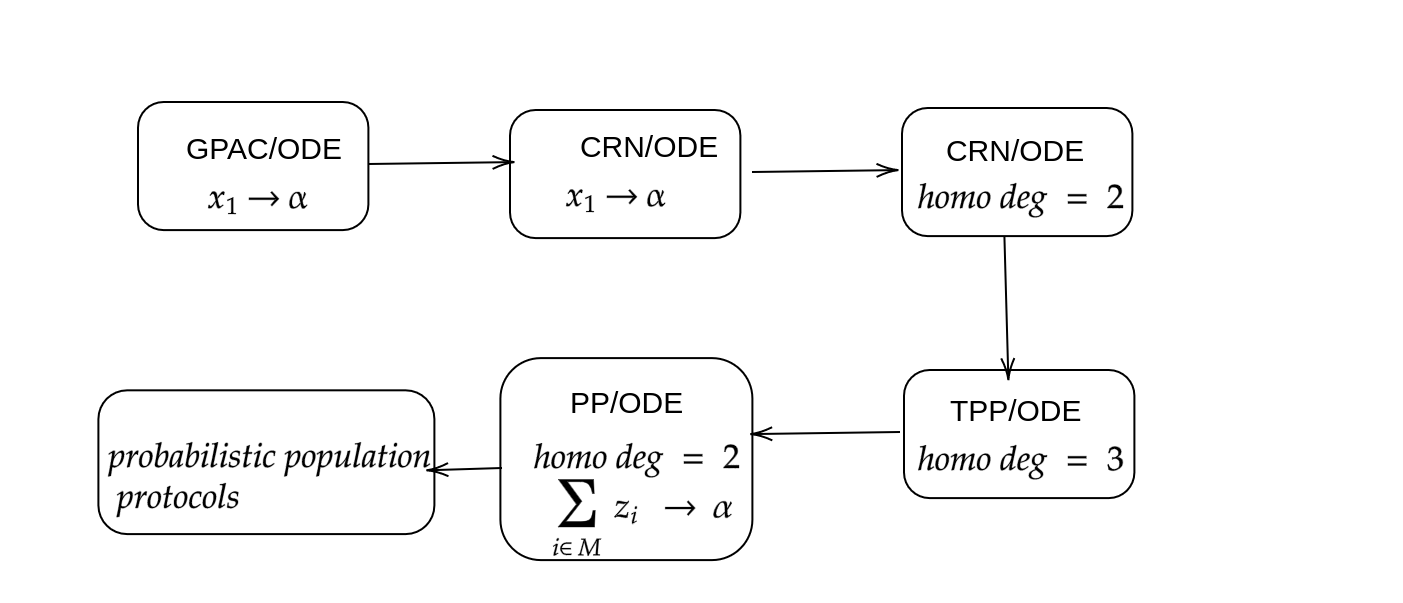
\includegraphics[scale=0.25]{flow-chart}
    \end{figure}
\end{frame}

\begin{frame}{The overview of the proof}
    \begin{figure}[tb]
        \centering
        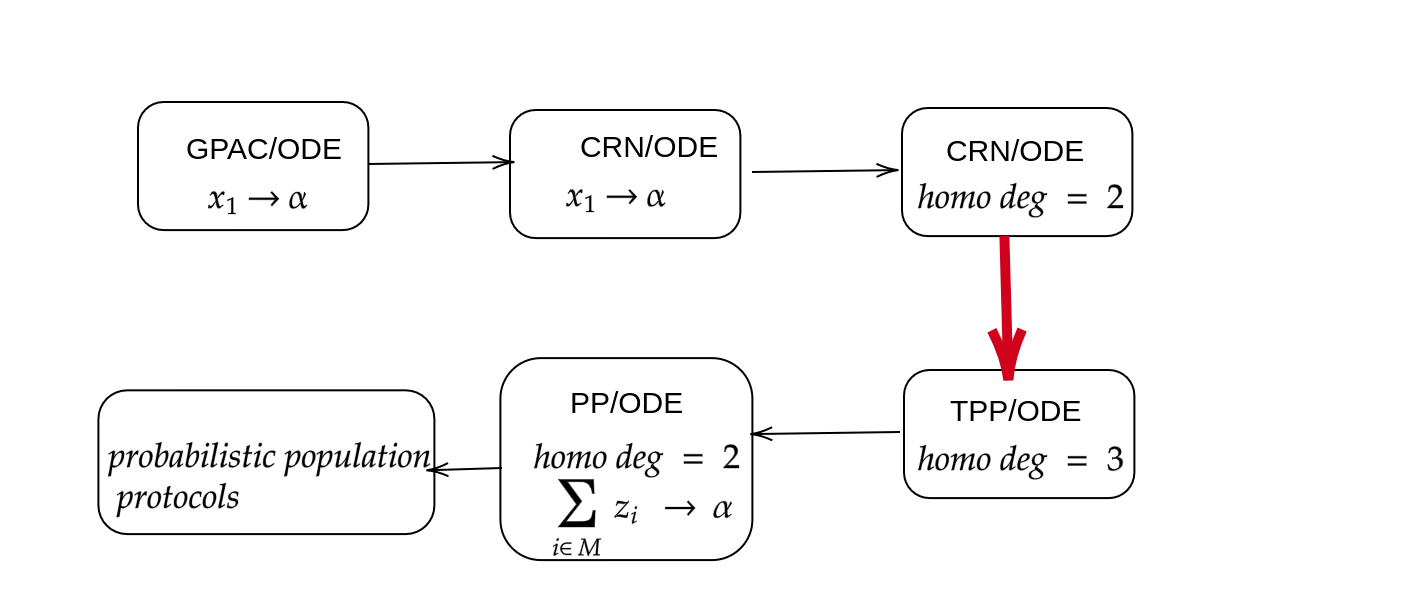
\includegraphics[scale=0.25]{flow2}
    \end{figure}
\end{frame}

\begin{frame}{A straightforward idea}
    A PP preserves population/mass.

    \begin{quest}
        Given a CRN $\bx=(x_1,\cdots, x_n)$, how could we make it preserve population/mass?
    \end{quest}\pause
    \begin{itemize}
        \item add a new variable $x_0$. \pause
        \item make the derivative of the new variable cancel all other change!
        \[
            x_0' = \sum_{i=1}^{n}x_i'
        \]
    \end{itemize}
\end{frame}
\begin{frame}[Clean]{A decent idea, but not work}
    $$ S= \begin{cases} dx_1 = \epsilon (a_0 + a_1 x_1 +\sum_{i=1}^{\delta-1}\frac{a_{i+1}}{\lambda^{i-1}}x_1x_i) \\ \\  dx_i = \lambda x_1 x_{i-1}-x_i \quad\text{ for } i=2,\dots,\delta-1           \\ \\ dx_\delta = -\sum_{i=1}^{\delta-1}dx_i \end{cases}$$\pause
    Bournez et. al. use this system to compute arbitrary \emph{algebraic} number. But the last summation bring in all the terms in the system, which is usually not implementable by PP.

    For example, $\sqrt{3}-\sqrt{2} $ with minimal polynomial $x^4-10x^2+1$ is a counterexample of their construction.
\end{frame}
\begin{frame}{$\sqrt{3}-\sqrt{2}$ }
    Let $(x_1,x_2,x_2,x_4)=(x,x^2,x^3,x^4)$. To encode the minimal polynomial, we have
    \[
        \left\{\begin{matrix}
x_1' &=  \;\;\;\;\;\, (x_4+1) - 10 x_1x_1
\\
x_2'&=  2x_1 ( x_4 + 1) -20x_1x_2
\\
x_3 ' &=  3x_2 ( x_4 + 1) -30x_1x_3
\\
x_4'  &=  4x_3 ( x_4 + 1) -40x_1x_4
\end{matrix}\right\}
    \]
\end{frame}

\begin{frame}[Clean]{Second attempt: TPP}
    We \emph{multiply} the variable we are going to introduce to the system.
    \[
        \left\{\begin{aligned}
x_1' &=   x_0\left[\;\;\;\;\;\,(x_4+1) - 10 x_1x_1\right]
\\
x_2'&=  x_0\left[2x_1 ( x_4 + 1) -20x_1x_2\right]
\\
x_3 ' &=  x_0\left[3x_2 ( x_4 + 1) -30x_1x_3\right]
\\
x_4'  &=  x_0\left[4x_3 ( x_4 + 1) -40x_1x_4\right]
\\
x_0'    &= -\sum\limits_{i=1}^4
x_i'\end{aligned}\right\}
    \]
\begin{itemize}
    \item every negative term of $x_0'$ now always has $x_0$.
    \item but now the system is of degree 3 (termolecular system)!
    \item $x_0'$ does not have positive $x_0^3$ term.
\end{itemize}
\end{frame}
\begin{frame}{TPP}
    \begin{figure}[tb]
        \centering
        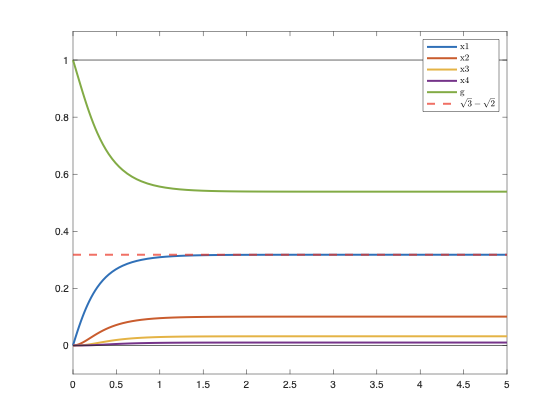
\includegraphics[scale=0.45]{tpp}
    \end{figure}
\end{frame}

\begin{frame}[Clean]{Time Dilation / Chain Rule}
But what is $x_0$ doing here?

Let $\bx(t)$ be the solution of $\bx' = p(\bx)$, where $\bx=(x_1, \cdots, x_n)$ be a vector of variables, $p$ a multivariable polynomial.
\begin{columns}
\begin{column}{0.5\textwidth}
   \begin{example}[Constant Dilation]
 Then x(2t) is the solution of the ODE:
    \[
        \bx'(t) = p(\bx) \cdot 2
    \]
\end{example}
\end{column}
\begin{column}{0.5\textwidth}  %%<--- here
\begin{example}[with a known function]
  Then x(F(t)) is the solution of the ODE:
  \[
        \bx'(t) = p(\bx) \cdot f(t),
  \]
  where $F(t)' = f(t)$.

  In our setting $F(t) =\int_{0}^{t} f(t) dt$
\end{example}
\end{column}
\end{columns}
\end{frame}

\begin{frame}[Clean]{Balancing Dilation}
\[
\begin{cases}
  x_i' = (p_i - q_i \cdot x_i)\cdot x_0,  \quad \text{for $i\in\{1, \cdots, n\}$}\\
  x_0' = -\sum_{i=1}^{n} x_i'.
\end{cases}
\]
\begin{itemize}
    \item The function $x_0$ is not known in advance.
    \item It is determined by the ODE above.
    \item How time dilates depends on / customizes to the original system $\bx$.
    \item The behavior of the new system at time $t$ corresponds to that of the old system at time $\int_0^{t}x_0(t)dt$.
    \item As long as $\int_0^{\infty}x_0 = \infty$, the new solution
    \[
        x_1(\int_0^{t}x_0) \to \alpha \quad\text{as $t\to\infty$.}
    \]
\end{itemize}
\end{frame}

\begin{frame}[Clean]{To Population Protocols}
    We now turn the TPP into PP.
    \begin{figure}[tb]
        \centering
        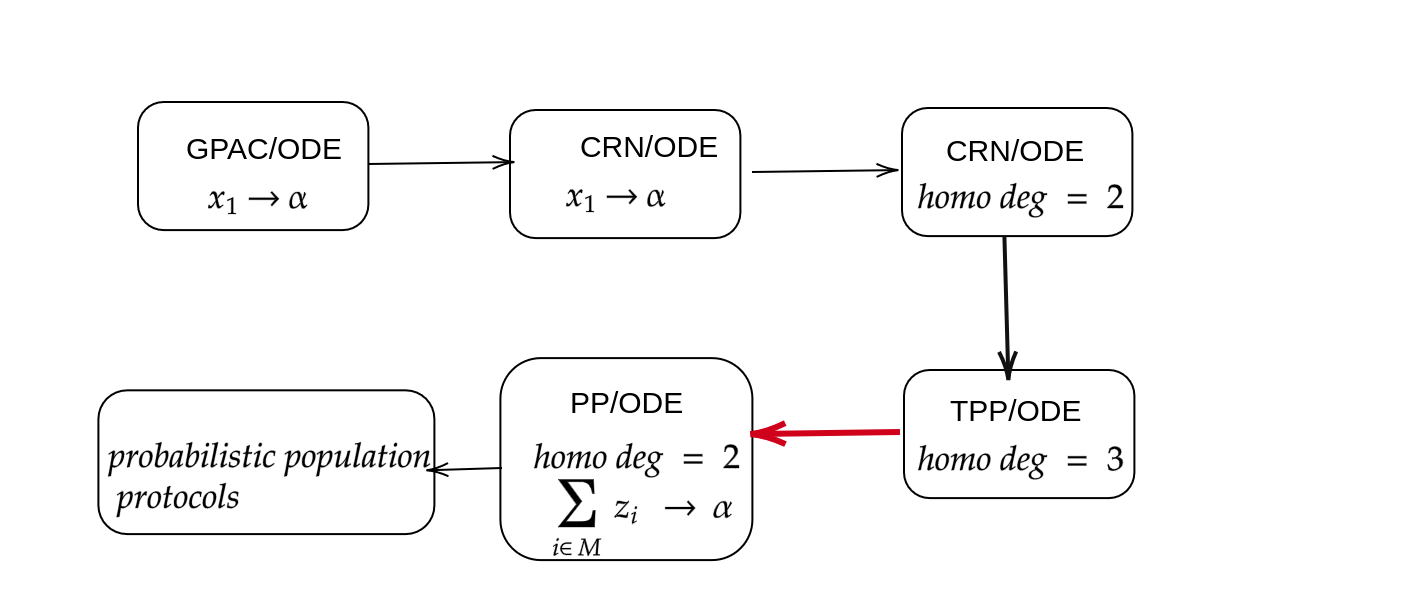
\includegraphics[scale=0.25]{flow3}
    \end{figure}
\end{frame}

\begin{frame}[Clean]{Calculus I again}
    We introduce
    \[
        z_{i,j} = x_i \cdot x_j
    \]
    Then
    \[
        z_{i,j}' = x_i' \cdot x_j + x_i \cdot x_j'
    \]
    \begin{itemize}
        \item The z-system is now of degree 4, homogeneously.
        \item Each term has the form such $x_1 x_2 x_4 x_5$, carefully assign the z-variable can make the system population-protocol implementable.
        \begin{itemize}
            \item Make sure it is CRN implementable first.
            \item Then avoid $z_{i,j}^2$ term in $z_{i,j}'$.
        \end{itemize}
     $x_1 x_2 x_4 x_5 = z_{1,2} \cdot z_{4,5}$ = $ z_{2,4}\cdot z_{1,5}$, etc.
    \end{itemize}
\end{frame}
\begin{frame}{Cont.}
We then have
    \begin{itemize}
        \item $x_1 = \displaystyle\sum_{j=0}^{n} z_{1,j}$. That is, the sum of $z_{1,j}$ trace the value of $x_1$. Hence computes $\alpha$.
        \item The z-system is implementable by population protocol.
    \end{itemize}
\end{frame}
\section{Future work}
\begin{frame}{Hierarchy down}
    GPAC/CRN/PP compute roughly the same set of real numbers. How about weaker models?

    \begin{example}[One-side protocols]
    The model with all the reactions in the form of:\\
    \[
         Y + X \to Z + X
    \]
    \end{example}
\end{frame}
\begin{frame}[Clean]{Hierarchy Up}
\begin{tabular}[t]{ll}
  \begin{minipage}{0.5\linewidth}
\centering
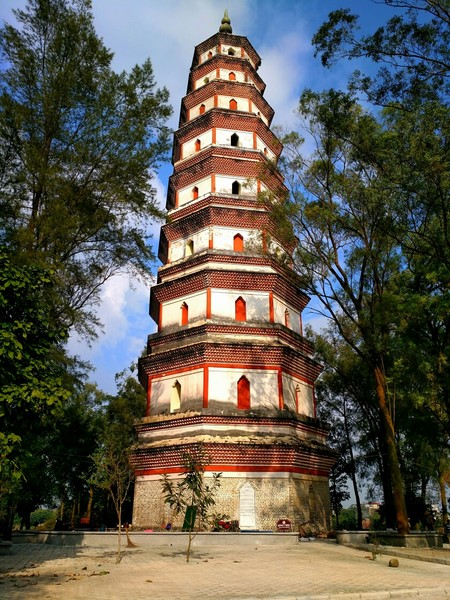
\includegraphics[scale=0.25]{dongta}
\end{minipage} &
\begin{minipage}{0.5\linewidth}
\centering
\begin{gather*}
  \vdots \\
  R_2=CRN(R_1)\\
  R_1=CRN(R_0)\\
  R_0= CRN(\Q) =GPAC(\Q) = PP(\Q).
\end{gather*}
We begin with allowing rational number as initial values and rate constants. Then build a new hierarchy on top the the previous level. \pause
\end{minipage}
\end{tabular}

\textbf{Question:} Do we really have a tower, or all layers collapse to $\R_0$? Or
\[
    R_0 \stackrel{?}{=} \bigcup_{i=0}^{\infty}R_i.
\]
\end{frame}

\begin{frame}
    \huge{Thank you for your time!}

    \vspace{0.5cm}
    \normalsize{}
    \begin{itemize}
        \item This research was supported in part by NSF grants 1545028 and 1900716.
        \item Rachel N. Huls : This research was supported in part by the University of Illinois Springfield Leadership Lived Experience (LLE) initiative.
    \end{itemize}
\end{frame}

\end{document}
